\chapter{Heurística: Colonia de Abejas Artificiales}

Una fuerte característica del ser humano es su forma de proceder 
para resolver problemas. En las Ciencias de la Computación, 
la problemática de encontrar una respuesta incluye el camino de 
describir la forma de resolverlo. En este capítulo se abordan algunas formas de 
hacer que la computadora ejecute dicho camino y se discute una descripción 
que se implementa como método de solución.

\section{Algoritmos}

Suponga que una persona va al supermercado y crea una lista con todos los
productos de su carrito. Cada producto tiene asociado un precio y se desea
averiguar si el total del carrito es menor o igual a la cantidad de dinero
disponible para efectuar la compra. ¿Cuál sería un método de solución
adecuado para este problema? Aunque pareciera que el problema es muy fácil
de resolver, el nivel de detalle que deben tener las indicaciones y pasos asociados a
la solución, posiblemente no son triviales de enunciar para una persona que nunca
ha descrito estos procesos a una computadora:

\begin{itemize}

\item \textbf{Input:} $L = $ Una lista de números que representan el precio de
  cada producto y un número $N$ el cual representa el límite de gastos.

\item \textbf{Output:} Un valor booleano de \texttt{TRUE} si la suma de los
  valores del carrito es menor o igual al número $N$, \texttt{FALSE} en caso
  contrario.

\end{itemize}

\begin{algorithm}
  \begin{algorithmic}[1]
    \Procedure{SumaMenorQue}{$L$, $N$}
      \State $N \leftarrow N -$ \textsc{SacaPrimero}($L$)
      \While{\textbf{true}}
        \If{$N < 0$}
          \State \textbf{return false}
        \EndIf
        \If{\textsc{EsVacio($L$)}}
          \State \textbf{return true}
        \EndIf
        \State $N \leftarrow N -$ \textsc{SacaPrimero}($L$)
      \EndWhile
    \EndProcedure
  \end{algorithmic}
  \caption{Algoritmo \textsc{SumaMenorQue}.}
  \label{code:algoritmo}
\end{algorithm}

Para llegar a la solución de un problema, una persona utiliza muchas veces
el instinto que va desarrollando a los largo de los años para analizar,
atacar y ejecutar un proceso que da una solución. Si se intenta
transmitir dicha técnica a una computadora, la manera más fácil de realizarlo
es mediante un proceso llamado \textit{algoritmo}.
Se puede decir informalmente que un algoritmo es cualquier procedimiento bien
definido que toma algún valor, o conjunto de valores como entrada
(o \textbf{Input}) y produce algún valor, o conjunto de valores como
salida (u \textbf{Output})~\cite{Cormen}. El análisis del problema en conjunto
a la abstracción de los objetos asociados y el resultado, producen
una serie de instrucciones que si se siguen correctamente, bajo una entrada
$I$, siempre regresará una salida $O$.

La investigación sobre la formalización de la definición de la palabra
\textit{algoritmo} sigue siendo motivo de estudio hasta nuestros días~\cite{Buss}.
Debido a los distintos tipos de problemas a resolver, existen muy diferentes
procesos, entradas y salidas que se pueden producir. Muchas veces existe más
de un algoritmo para resolver el mismo problema y algunos de ellos producen una
salida de manera más óptima que otros\footnote{En este caso, el factor para
que un algoritmo es más eficiente que otro se basa en la complejidad
en espacio o tiempo (\textit{big-O}).} . La llamada ``caracterización'' de los algoritmos
es algo que se ha discutido por más de doscientos años; un ejemplo de esto
es el algoritmo de la criba de Eratóstenes que nos permite hallar todos los
números primos menores a un número natural $m$ dado.

Para propósitos de esta tesis, la definición informal que se usará será la
siguiente: \textbf{Un algoritmo es una secuencia de pasos bien definida y finita
  tal que dada una entrada $I$, produce siempre la salida $O$}. Se considerará
que los algoritmos deben tener también la característica de finitud
(\cite{Physics},~\cite{Rogers1967}~y~\cite{Cormen}).

Así como existen problemas en los que escribir el algoritmo para encontrar
la solución resulta sencillo y el proceso descrito pueda verse fácilmente
eficiente (como el~\Cref{code:algoritmo}), existen problemas en los que
dar la descripción para obtener la mejor solución no es una opción práctica.

\subsection{\texttt{3-SAT}}

Sea el problema \texttt{3SAT}, el cual consiste en dado un conjunto de fórmulas
$\phi = \{x_{1}, x_{2}, x_{3}, ..., x_{n}\}$ con cada $x_{i}$ una fórmula lógica
de la forma $x_{i} = p_{i} \lor q_{i} \lor r_{i} $, con $ p_{i}, q_{i}, r_{i}$,
variables o términos lógicos, se deberá encontrar una
interpretación $\mathcal{I}$ tal que $\mathcal{I}(\phi) = \mathcal{I}(x_{i}) = 1$
$\forall i \in \{1,2,...,n\}$. Existen algoritmos para resolver este problema
y similares\footnote{Recordar que en el capítulo 2 se aborda la equivalencia de
los problemas \textsl{NP}-completos.}, sin embargo, su complejidad en tiempo es de la
forma $O(X^{n})$ con $3|\phi| = n$ y $X$ una constante~\cite{Marques-Silva}.

Para propósitos demostrativos, se ha creado un algoritmo de búsqueda exhaustiva.
El código que se encuentra en el \cref{apendice:sat} sirve para correr
ejemplos de fórmulas y encontrar interpretaciones en las que el valor de
verdad de la fórmula sea \texttt{TRUE} (o~1). En caso de que no exista una
interpretación verdadera, el programa implementado regresa el mensaje de que no se pudo
realizar una asignación (lo que sería equivalente al valor de \texttt{FALSE} en \texttt{3-SAT}):

\begin{figure}[h]
\begin{displaymath} 
\mathcal{I}(s \lor j \lor \neg z) =\left\{
  \begin{array}{rcl}
    \mathcal{I}(s) & = & \texttt{FALSE} \\
    \mathcal{I}(j) & = & \texttt{FALSE}  \\
    \mathcal{I}(z) & = & \texttt{FALSE} 
  \end{array}
  \right.
\end{displaymath}
\caption[short caption]{Salida del programa en el \cref{apendice:sat}.}
\label{fig:salida1}
\end{figure} 

Se puede ver que $\mathcal{I}(\phi) = 1$ con la asignación de la \Cref{fig:salida1} 
ya que $\mathcal{I}(z) = 0 \rightarrow \mathcal{I}(\neg z) = 1$ y
por lo tanto, $\mathcal{I}(s \lor j \lor \neg z) = 1$.

Con este mismo programa se puede forzar una fórmula que no tenga solución y así
realizar el cálculo de todas las posibles combinaciones de asignaciones.
Si se agrega  como parámetro \texttt{--no-solucion}, el programa agregará el
siguiente conjunto $\phi_{imp}$ de cláusulas al programa, definido en \Cref{tab:3sat}.

\begin{table}[h]
\[
\small
\centering
\begin{array}{C|C|C|C|C|C|C}
$P$ & $Q$ & $R$ & $\overbrace{(P \lor Q \lor R)}^{\textbf{(a)}}$ & $\overbrace{(\neg P \lor Q \lor R)}^{\textbf{(b)}}$ & $\overbrace{(P \lor \neg Q \lor R)}^{\textbf{(c)}}$ & $\overbrace{(P \lor Q \lor \neg R)}^{\textbf{(d)}}$  \\
\hline
T & T & T & T & T & T & T \\
T & T & F & T & T & T & T \\
T & F & T & T & T & T & T \\
T & F & F & T & F & T & T \\
F & T & T & T & T & T & T \\
F & T & F & T & T & F & T \\
F & F & T & T & T & T & F \\
F & F & F & F & T & T & T
\end{array}
\]

\[
\small
\centering
\begin{array}{C|C|C|C|C|C|C}
$P$ & $Q$ & $R$ & $\overbrace{(\neg P \lor \neg Q \lor R)}^{\textbf{(e)}}$ & $\overbrace{(\neg P \lor Q \lor \neg R)}^{\textbf{(f)}}$ & $\overbrace{(P \lor \neg Q \lor \neg R)}^{\textbf{(g)}}$ & $\overbrace{(\neg P \lor \neg Q \lor \neg R)}^{\textbf{(h)}}$  \\
\hline
T & T & T & T & T & T & F \\
T & T & F & F & T & T & T \\
T & F & T & T & F & T & T \\
T & F & F & T & T & T & T \\
F & T & T & T & T & F & T \\
F & T & F & T & T & T & T \\
F & F & T & T & T & T & T \\
F & F & F & T & T & T & T
\end{array}
\]
\caption{Tabla de verdad con las fórmulas de todas las posibles combinaciones de tres variables $P$, $Q$ y $R$ en la forma normal conjuntiva \textit{(NFC)}.\label{tab:3sat}}
\end{table}

Como se puede observar en la tabla \Cref{tab:3sat}, existe siempre para alguna
combinación de valores de $P$, $Q$ y $R$, el valor de $F$ (o falso) en todas
las columnas y filas, por lo tanto, como se ve en la tabla \ref{tab:3sat2}, se puede
suponer que $\nexists~\mathcal{I} \mid \mathcal{I}(\phi_{imp}) = 1$.

\begin{table}
\[
\centering
\begin{array}{C|C|C|C}
$P$ & $Q$ & $R$ & $ (a) \land (b)  \land (c)  \land (d)  \land (e)  \land (f)  \land (g)  \land (h)  $  \\
\hline
T & T & T & F \\
T & T & F & F \\
T & F & T & F \\
T & F & F & F \\
F & T & T & F \\
F & T & F & F \\
F & F & T & F \\
F & F & F & F
\end{array}
\]
\caption{Tabla de verdad con las conjunciones del resultado de la
tabla \Cref{tab:3sat}.} \label{tab:3sat2}
\end{table}

\begin{center}
  \begin{minipage}{1.0\textwidth}
    \begin{lstlisting}[caption={Ejecución de una fórmula sin solución.}\label{code:3sat-no-solucion1},captionpos=b]
      (*@
      \begin{commandshell}
        # python sat.py --no-solucion
        No se pudo realizar asignación, se intentó 1 fórmula(s).
        Num de asignaciones que se realizaron: 14
      \end{commandshell}
      @*)
    \end{lstlisting}
  \end{minipage}
\end{center}


Al no existir una posible combinación para este conjunto de fórmulas, el
algoritmo en el~\cref{apendice:sat} asignará todas las posibles combinaciones de
valores a cada una de las variables; para tres variables el número de
asignaciones que se realizan es 14, que es el resultado de la suma del total de las
llamadas recursivas y es el número total de aristas en el árbol de búsqueda. El
hecho de que el árbol sea binario depende sólo de que existan dos posibles valores
de verdad para cada variable.

\begin{figure}[H]
\centering
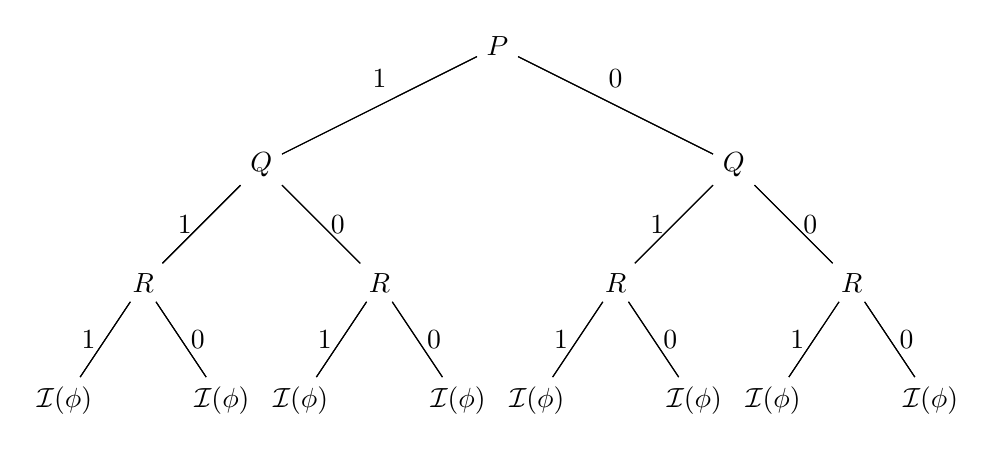
\begin{tikzpicture}[level/.style={sibling distance=60mm/#1}]
  \node (a) {$P$}
    child {node (b) {$Q$}
      child {node (d) {$R$}
      	child {node (dl) {$\mathcal{I}(\phi)$}}
      	child {node (dr) {$\mathcal{I}(\phi)$}}
      	}
      child {node (e) {$R$}
      	child {node (el) {$\mathcal{I}(\phi)$}}
      	child {node (er) {$\mathcal{I}(\phi)$}}
      	}
    }
    child {node (c) {$Q$}
    child {node (f) {$R$}
    	child {node (fl) {$\mathcal{I}(\phi)$}}
    	child {node (fr) {$\mathcal{I}(\phi)$}}
    	}
      child {node (g) {$R$}
      	child {node (gl) {$\mathcal{I}(\phi)$}}
      	child {node (gr) {$\mathcal{I}(\phi)$}}
      	}
    }; 	
%\path (a) -- (b) node {TRUE};
\path (a) edge node[above=3pt]{$1$} (b);
\path (a) edge node[above=3pt]{$0$} (c);

\path (b) edge node[left]{$1$} (d);
\path (b) edge node[right]{$0$} (e);
\path (c) edge node[left]{$1$} (f);
\path (c) edge node[right]{$0$} (g);

\path (d) edge node[left]{$1$} (dl);
\path (d) edge node[right]{$0$} (dr);
\path (e) edge node[left]{$1$} (el);
\path (e) edge node[right]{$0$} (er);
\path (f) edge node[left]{$1$} (fl);
\path (f) edge node[right]{$0$} (fr);
\path (g) edge node[left]{$1$} (gl);
\path (g) edge node[right]{$0$} (gr);
\end{tikzpicture}
\caption{Árbol de asignaciones de valores con tres variables.} \label{fig:a3sat01}
\end{figure}

Para una cláusula con tres variables, el árbol realiza 14 asignaciones, para
dos cláusulas con seis variables el árbol tendrá 126 aristas representando
las asignaciones, para tres claúsulas $1,022$ y para 21 variables el número se eleva
a $4,194,302$. Para 33 variables (u once cláusulas) se corrió el programa durante más de
un día debido a que el árbol es demasiado grande para revisar todas las asignaciones en
menos de 24 horas\footnote{Se realizó la experimentación y se hizo el total de 
asignaciones en 26 horas con 25 minutos y 41 segundos.}\footnote{El número obtenido fue $17,179,869,182$ (diecisiete mil
ciento setenta y nueve millones ochocientos sesenta y nueve mil ciento ochenta
y dos).}.

\begin{figure}[h]
% GNUPLOT: LaTeX picture
\setlength{\unitlength}{0.240900pt}
\ifx\plotpoint\undefined\newsavebox{\plotpoint}\fi
\sbox{\plotpoint}{\rule[-0.200pt]{0.400pt}{0.400pt}}%
\begin{picture}(1500,900)(0,0)
\sbox{\plotpoint}{\rule[-0.200pt]{0.400pt}{0.400pt}}%
\put(171.0,131.0){\rule[-0.200pt]{4.818pt}{0.400pt}}
\put(151,131){\makebox(0,0)[r]{$0$}}
\put(1419.0,131.0){\rule[-0.200pt]{4.818pt}{0.400pt}}
\put(171.0,313.0){\rule[-0.200pt]{4.818pt}{0.400pt}}
\put(151,313){\makebox(0,0)[r]{$500$}}
\put(1419.0,313.0){\rule[-0.200pt]{4.818pt}{0.400pt}}
\put(171.0,495.0){\rule[-0.200pt]{4.818pt}{0.400pt}}
\put(151,495){\makebox(0,0)[r]{$1,000$}}
\put(1419.0,495.0){\rule[-0.200pt]{4.818pt}{0.400pt}}
\put(171.0,677.0){\rule[-0.200pt]{4.818pt}{0.400pt}}
\put(151,677){\makebox(0,0)[r]{$1,500$}}
\put(1419.0,677.0){\rule[-0.200pt]{4.818pt}{0.400pt}}
\put(171.0,859.0){\rule[-0.200pt]{4.818pt}{0.400pt}}
\put(151,859){\makebox(0,0)[r]{$2,000$}}
\put(1419.0,859.0){\rule[-0.200pt]{4.818pt}{0.400pt}}
\put(171.0,131.0){\rule[-0.200pt]{0.400pt}{4.818pt}}
\put(171,90){\makebox(0,0){$2$}}
\put(171.0,839.0){\rule[-0.200pt]{0.400pt}{4.818pt}}
\put(488.0,131.0){\rule[-0.200pt]{0.400pt}{4.818pt}}
\put(488,90){\makebox(0,0){$3$}}
\put(488.0,839.0){\rule[-0.200pt]{0.400pt}{4.818pt}}
\put(805.0,131.0){\rule[-0.200pt]{0.400pt}{4.818pt}}
\put(805,90){\makebox(0,0){$4$}}
\put(805.0,839.0){\rule[-0.200pt]{0.400pt}{4.818pt}}
\put(1122.0,131.0){\rule[-0.200pt]{0.400pt}{4.818pt}}
\put(1122,90){\makebox(0,0){$5$}}
\put(1122.0,839.0){\rule[-0.200pt]{0.400pt}{4.818pt}}
\put(1439.0,131.0){\rule[-0.200pt]{0.400pt}{4.818pt}}
\put(1439,90){\makebox(0,0){$6$}}
\put(1439.0,839.0){\rule[-0.200pt]{0.400pt}{4.818pt}}
\put(171.0,131.0){\rule[-0.200pt]{0.400pt}{175.375pt}}
\put(171.0,131.0){\rule[-0.200pt]{305.461pt}{0.400pt}}
\put(1439.0,131.0){\rule[-0.200pt]{0.400pt}{175.375pt}}
\put(171.0,859.0){\rule[-0.200pt]{305.461pt}{0.400pt}}
\put(30,495){\rotatebox{90}{\makebox(0,0){Asignaciones}}
}\put(805,29){\makebox(0,0){Fórmulas}}
\put(488,136){\usebox{\plotpoint}}
\multiput(488.00,136.58)(3.894,0.498){79}{\rule{3.193pt}{0.120pt}}
\multiput(488.00,135.17)(310.373,41.000){2}{\rule{1.596pt}{0.400pt}}
\multiput(805.58,177.00)(0.500,0.514){631}{\rule{0.120pt}{0.511pt}}
\multiput(804.17,177.00)(317.000,324.939){2}{\rule{0.400pt}{0.256pt}}
\put(488,136){\makebox(0,0){$+$}}
\put(805,177){\makebox(0,0){$+$}}
\put(1122,503){\makebox(0,0){$+$}}
\put(1122.0,503.0){\rule[-0.200pt]{0.400pt}{85.760pt}}
\put(171.0,131.0){\rule[-0.200pt]{0.400pt}{175.375pt}}
\put(171.0,131.0){\rule[-0.200pt]{305.461pt}{0.400pt}}
\put(1439.0,131.0){\rule[-0.200pt]{0.400pt}{175.375pt}}
\put(171.0,859.0){\rule[-0.200pt]{305.461pt}{0.400pt}}
\end{picture}

\caption[short caption]{Muestra del crecimiento de asignaciones respecto a las fórmulas de $\phi$.}
\label{fig:satfigure}
\end{figure} 


El algoritmo dado produce la solución (si es que existe) pero el costo en tiempo
es demasiado alto. Este algoritmo es lo que se le denomina de tiempo ``exponencial'' y
esto se debe a que el número de asignaciones crece de la siguiente manera (\Cref{fig:satfigure}):

\begin{figure}[H]
\centering
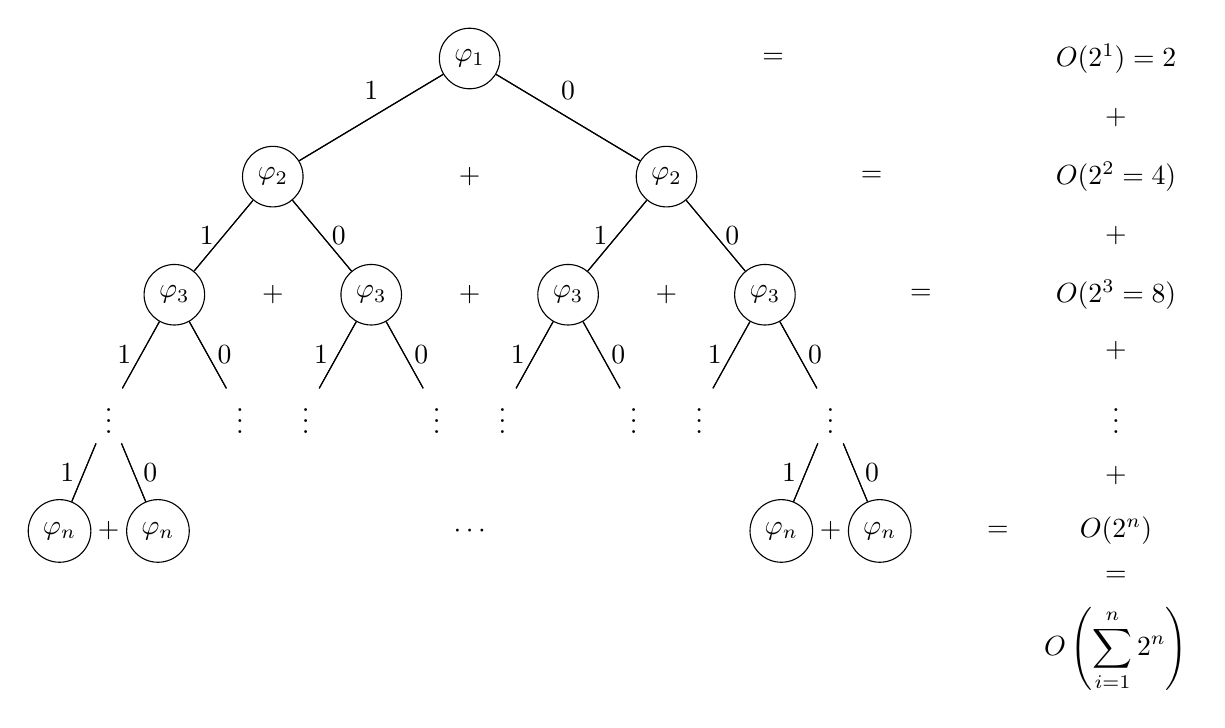
\begin{tikzpicture}[level/.style={sibling distance=50mm/#1}]
\node [circle,draw] (z){$\varphi_{1}$}
  child {node [circle,draw] (a) {$\varphi_{2}$}
    child {node [circle,draw] (b) {$\varphi_{3}$}
      child {node (p1) {$\vdots$}
        child {node [circle,draw] (d) {$\varphi_{n}$}}
        child {node [circle,draw] (e) {$\varphi_{n}$}}
      }
      child {node (p2) {$\vdots$}}
    }
    child {node [circle,draw] (g) {$\varphi_{3}$}
      child {node (p3) {$\vdots$}}
      child {node (p4) {$\vdots$}}
    }
  }
  child {node [circle,draw] (j) {$\varphi_{2}$}
    child {node [circle,draw] (k) {$\varphi_{3}$}
      child {node (p5) {$\vdots$}}
      child {node (p6) {$\vdots$}}
    }
  child {node [circle,draw] (l) {$\varphi_{3}$}
    child {node (p7) {$\vdots$}}
    child {node (c){$\vdots$}
      child {node [circle,draw] (o) {$\varphi_{n}$}}
      child {node [circle,draw] (p) {$\varphi_{n}$}
        child [grow=right] {node (q) {$=$} edge from parent[draw=none]
          child [grow=right] {node (q) {$O(2^{n})$} edge from parent[draw=none]
            child [grow=up] {node (r) {$\vdots$} edge from parent[draw=none]
              child [grow=up] {node (s) {$O(2^{3}=8)$} edge from parent[draw=none]
                child [grow=up] {node (t) {$O(2^{2}=4)$} edge from parent[draw=none]
                  child [grow=up] {node (u) {$O(2^{1})=2$} edge from parent[draw=none]}
                }
              }
            }
            child [grow=down] {node (v) {$O\left(\displaystyle\sum_{i = 1}^n 2^n \right)$}edge from parent[draw=none]}
          }
        }
      }
    }
  }
};
\path (a) -- (j) node [midway] {+};
\path (b) -- (g) node [midway] {+};
\path (k) -- (l) node [midway] {+};
\path (k) -- (g) node [midway] {+};
\path (d) -- (e) node [midway] {+};
\path (o) -- (p) node [midway] {+};
\path (o) -- (e) node (x) [midway] {$\cdots$};
\path (q) -- (r) node [midway] {+};
\path (s) -- (r) node [midway] {+};
\path (s) -- (t) node [midway] {+};
\path (s) -- (l) node [midway] {=};
\path (t) -- (u) node [midway] {+};
\path (z) -- (u) node [midway] {=};
\path (j) -- (t) node [midway] {=};
\path (q) -- (v) node [midway] {=};



\path (z) edge node[above=3pt]{$1$} (a);
\path (z) edge node[above=3pt]{$0$} (j);

\path (a) edge node[left]{$1$} (b);
\path (a) edge node[right]{$0$} (g);
\path (j) edge node[left]{$1$} (k);
\path (j) edge node[right]{$0$} (l);

\path (b) edge node[left]{$1$} (p1);
\path (b) edge node[right]{$0$} (p2);
\path (g) edge node[left]{$1$} (p3);
\path (g) edge node[right]{$0$} (p4);
\path (k) edge node[left]{$1$} (p5);
\path (k) edge node[right]{$0$} (p6);
\path (l) edge node[left]{$1$} (p7);
\path (l) edge node[right]{$0$} (c);

\path (p1) edge node[left]{$1$} (d);
\path (p1) edge node[right]{$0$} (e);
\path (c) edge node[left]{$1$} (o);
\path (c) edge node[right]{$0$} (p);

\end{tikzpicture}
\caption{Posibles valores de verdad por cada variable en un árbol binario.} \label{fig:a3sat02}
\end{figure}

En el 2010 se publicó un artículo donde describen un algoritmo que reduce la
complejidad a $O(1.439^{n})$ y existe una competencia anual que premia a las
mejores implementaciones para encontrar soluciones al problema
\texttt{SAT},\cite{Kutzkov2010} \cite{satcompetition}, sin embargo las
soluciones siguen siendo exponenciales.  Habría que mencionar que si se
encuentra una solución en tiempo \textsl{P} se estaría demostrando que
$\textsl{P}=\textsl{NP}$.

\section{Heurísticas}

Una alternativa a solucionar problemas como \texttt{3-SAT} o
equivalentes\footnote{Que sea un problema perteneciente a la clase \textsl{NP} o
  con una cota \textit{$big-O$} que se quisiera reducir.} son estrategias y procesos
que se utilizan fácilmente debido a la información libremente aplicada para
controlar los procesos de resolución de problemas en máquinas. Estos procesos
son criterios, métodos o principios para decidir cuál de los varios cursos de
acción alternativos promete ser el más eficaz para lograr algún objetivo. Estos
procesos reciben el nombre de \textbf{heurísticas}~\cite{Pearl1984}.

A diferencia de los algoritmos\footnote{En algunos textos
  como~\cite{DeInformatica2010} se le llaman a las heurísticas
  \textit{algoritmos heurísticos}.} informalmente definidos previamente, las
heurísticas también son una secuencia de pasos bien definida pero dada una
entrada $I$, produce una salida $o \in \texttt{OUTPUT}$ con $\texttt{OUTPUT}$ un
conjunto de posibles valores de solución.  Las respuestas dadas por las
heurísticas normalmente no suelen ser la mejor solución, pero intentan producir
una solución \emph{suficientemente buena}~\cite{Gigerenzer2008}.  Generalmente
sus salidas son el resultado de ejecuciones de funciones estocásticas y
raramente almacenan información del proceso de obtención del resultado
previo~\cite{heuristicdefoxford},\cite{Pearl1984}.

Las heurísticas son tan diversas que es difícil clasificarlas exclusivamente en sólo 
una categoría, sin embargo existen características que comparten ciertas heurísticas:
los métodos resolutivos llamados de \textit{búsqueda tabú} son aquellos que determinan 
una posible respuesta, las marcan y premian la exploración de soluciones alejadas de las 
posibles respuestas marcadas. Los algoritmos (heurísticos) genéticos están por su parte 
inspirados en la evolución biológica, modificando poblaciones (de objetos a mejorar) y 
premiando a las soluciones más cercanas al objetivo. Existen muchos otras heurísticas como 
las redes neuronales o reocido simulado y si bien todas diferentes, comparten la 
característica de producir soluciones sin garantizar necesariamente que sea la mejor.

Cuando se habla de heurísticas, es importante mencionar que en algunos
textos~\cite{Pearl1984} hablan sobre una cierta \textit{intuición} o criterio
cuando se refiere al plantearlas como métodos resolutivos, por
los que en algunas ocasiones es difícil entender el \textit{``¿por qué
  funciona?''}; se propone que la intuición mencionada es la capacidad de hacer
predicción sobre un conjunto de datos o la eliminación de información previa
innecesaria (o ``ruido'')~\cite{Gigerenzer2008}.

\subsection{El problema de las 8 reinas}

Franz Nauck publicó en 1850 un (ahora) famoso problema para el matemático Gauss:
el problema consiste en obtener el método para determinar cómo ocho reinas
pueden ser colocadas en un tablero de ajedrez\footnote{El problema general es
  colocar $n$ reinas en un tablero de $n^{2}$ casillas.} de tal manera que una
reina no pueda \textit{tomar} a otra~\cite{RouseBall2008}. En otras palabras,
dos reinas no pueden estar colocadas en la misma columna, fila o diagonal.

\begin{figure}[H]
\centering
\medskip

\newgame
\fenboard{q7/6q1/4q3/7q/1q6/3q4/5q2/2q5 w - - 0 20}
\showboard
\caption{Ejemplo de solución al poblema de las 8 reinas.} \label{fig:t8rein01}
\end{figure}

Poco después del planteamiento (1848), este problema fue resuelto y aparecieron
un total de 40 soluciones entre los años 1849 y 1854 en la revista de ajedrez
alemana \textit{Deutsche Schachzeitung}~\cite{Campbell1977}.  El problema de las
8 reinas es, desde un punto de vista computacional, interesante de usar como 
ejemplo de un problema que es resuelto por una heurística, debido a que la 
versión generalizada del problema, de las $n$-reinas, es un problema 
\textsl{NP}-completo~\cite{Gent2017}.

Como muestra de la aplicación de una heurística, se implementó un conjunto de
funciones que usan una función de costo, una entrada y un factor aleatorio para
hayar soluciones al problema de las reinas. El código se puede leer
en el~\Cref{apendice:reinas}. La función de costo y funcionamiento de la
heurística es la que se muestra a continuación.

La secuencia de ordenamiento de reinas no es aleatorio sino sistemático, de
esta manera se asegura que no se genera la misma combinación de posiciones una
y otra vez eficientando la heurística. Al no crear las mismas combinaciones
se tendrá más probabilidad de éxito de generar alguna combinación deseada.
Una forma de sistematizar el generamiento de posiciones de las reinas es
colocándolas una a la vez empezando con un tablero vacío, hasta que todas
estén colocadas.

Para poder asignar las reinas se debe tener en consideración que dada una reina
puesta con anterioridad, se reduce el número de casillas donde puede ser colocada
sin correr el riesgo de ser ``tomada'' por otra reina. Una casilla es candidata
a ser asignada a una reina prioritariamente si al colocarla, ésta deja un número
alto de casillas ``no atacadas'', esto es, que deja la mayor cantidad de
casillas para la posterior asignación del resto de las reinas. Aquí hay un
ejemplo:

\begin{figure}[H]
\centering
\medskip
\newgame
\fenboard{3q4/1q6/7q/2Q1QQ2/8/8/8/8 w - - 0 20}
\showboard
\caption{Problemática de asignación de una reina en C5, E5 o F5.} \label{fig:t8rein02}
\end{figure}

Considérese a las reinas blancas como ``no asignadas''. Para la función de
costo, se utilizó como información el número de casillas donde se puedan colocar
reinas en la próxima iteración, tratando de maximizarlo para tener más
oportunidades de éxito. El numero de casillas que quedan se transforma en
el método de asignación:

\begin{displaymath}
  \begin{array}{rcl}
    f(c5) & = & 8 \\
    f(e5) & = & 9 \\
    f(f5) & = & 10.
  \end{array}
\end{displaymath}

La opción que la heurística tomaría en este caso sería aquella donde la reina
es asignada a la casilla $c5$. Algunas iteraciones llegan al caso donde
$f(X) = f(Y)$ y aquí es donde se realiza una asignación aleatoria y se escoge
cualquiera de las dos. Es posible que se llegue a un punto donde no se pueda
seguir asignando más reinas, en este caso la heurística vuelve a partir de cero
con un nuevo tablero.

\begin{figure}[H]
\centering
\medskip
\newgame
\fenboard{5q2/q7/4q3/1q6/7q/2q5/6q1/3q4 w - - 0 20}
\showboard
\caption{Resultado de la ejecución de la heurística de reinas con un tablero de 8 x 8.} \label{fig:t8rein03}
\end{figure}

\section{Aproximación numérica como solución a problemas \textsl{NP}}

La búsqueda de alternativas para resolver problemas no tratables de manera
frontal no es un tema nuevo: en 1739 fueron publicadas varias notas de Sir
Isaac Newton, las cuales contienen un método para encontrar aproximaciones de
raíces a funciones. El método de Newton converge sólo bajo ciertas condiciones;
sin estas condiciones el procedimiento fácilmente podría alejarse del resultado
esperado~\cite{newton}. Para obtener soluciones \textit{buenas} dado un método,
hay que definir lo que significa \textit{bueno} y esto consiste en un conjunto
de condiciones y reglas que servirán para acotar algún resultado previamente
definido.

En matemáticas, los métodos de optimización son aquellos que consisten en
maximizar o minimizar una función por cada iteración, manipulando los valores
dentro de un dominio definido para aproximar a algún objetivo. Los problemas de
optimización tienen la forma:

\begin{displaymath}
  \min f_{0}(x), ~ \textrm{sujeto a} ~ f_{i}(x) \leq b_{i}, i = 1,...,m,
\end{displaymath}

\noindent donde el vector $x=(x_{1},...,x_{n})$ es la variable de optimización
del problema; la función $f_{0}: \mathbb{R}^{n} \rightarrow \mathbb{R}$ es la
función de costo u objetivo; las funciones
$f_{i}: \mathbb{R}^{n} \rightarrow \mathbb{R}$, $i = 1,...,m$, son de
restricción y las constantes $b_{1},...,b_{m}$ son los valores límites para las
funciones de restricción. Se dice que un vector $x^{*}$ es óptimo (o una
solución del problema) si tiene el menor (o mayor en caso de maximizar) valor objetivo de todos los vectores
que satisfacen el límite; para todo $z$ con
$f_{1}(z) \leq b_{1}, ..., f_{m}(z) \leq b_{m}$, se tiene que
$f_{0}(z) \geq f_{0}(x^{*})$~\cite{Boyd:2004:CO:993483}.

En Ciencias de la Computación, los algoritmos de aproximación y heurísticas
numéricas son métodos de resolución (generalmente a problemas \textsl{NP}), que
aunque no proveen de \textit{puntos de apoyo} para encontrar la mejor solución,
sí ofrecen estos puntos para obtener soluciones que se \emph{aproximan} a la
óptima de manera eficiente. Estos métodos de resolución parten de la conjetura
de $\textsl{P} \neq \textsl{NP}$ para aseverar su
eficiencia~\cite{Vazirani:2001:AA:500776}.

A diferencia de los algoritmos de aproximación, las heurísticas no garantizan
un resultado dentro de una constante $c$ de factibilidad cercana al óptimo, ni
tienen que cumplir la condición de que termine en tiempo polinomial respecto
al tamaño de la entrada. Las heurísticas se pueden comportar de manera muy
pobre si se considera el peor caso, sumado a un subconjunto de instancias del
problema que harían su desempeño poco destacable. Sin embargo, buenas
heurísticas pueden superar el desempeño de muchos algoritmos con muchas
instancias~\cite{Ausiello:1999:CAC:554706}, reduciendo el espacio de búsqueda
de problemas (incluidos los de la clase \textsl{NP}-duro).

\section{Colonia de abejas artificiales}

La observación del comportamiento de enjambres ha ganado terreno en el interés
de los científicos debido a las formas particulares en las que estas comunidades
resuelven sus problemas. Dervis Karaboga enumera dos principales conceptos que
son necesarios para que los enjambres obtengan el comportamiento de
inteligencia: la organización del enjambre y la división de labores. Karaboga
describió en el año 2005 la heurística que se usa en esta tesis y que lleva como
nombre \textit{Colonia de abejas artificiales} o \textit{ABC}\footnote{Por sus
  iniciales en inglés \textit{Artificial Bee Colony.}}.

El modelo minimalista del comportamiento de una colonia de abejas real
que Keraboga describe como base del funcionamiento para su heurística
enumera una serie de agentes que tienen como propósito el emular condiciones
de un panal de abejas en la intemperie de forma artificial. Las funciones
principales están divididas tres componentes esenciales:

\begin{enumerate}
\item Fuente de alimentación: La fuente es un espacio abierto proveedor de
\textit{néctar} que puede o no estar delimitado por ciertas reglas. El valor
de la fuente fluctuará respecto a la rentabilidad de la solución.

\item Abejas recolectoras empleadas: Tienen asociada una fuente de alimentación que
consumen continuamente. Cada abeja \textit{contiene} la información de su
fuente.

\item Abejas recolectoras desempleadas: Buscan continuamente una fuente de
alimentación que consumir. Existen a su vez, dos tipos de abejas recolectoras
desempleadas:

\begin{enumerate}

\item Exploradoras: Son entre 5-10\% de la colmena. Exploran el espacio de búsqueda
para encontrar nuevas fuentes de alimento.

\item Observadoras: Esperan en la colmena y clasifican las fuentes de
alimentación con la información que provee el resto del enjambre.

\end{enumerate}
\end{enumerate}

Para que exista la organización como uno de los conceptos principales de un
enjambre, es necesario un proceso de comunicación. Como ocurre con las colmenas
de abejas en la naturaleza, Karaboga propone un área de \textit{baile}; este
baile que llama en inglés \textit{waggle dance} comunica a las abejas
observadoras el valor de la fuente y cada una puede decidir cuál fuente de
alimentación tiene la mejor valoración. Las abejas recolectoras empleadas
comparten su información en el área de baile junto a una probabilidad
proporcional a la rentabilidad de la fuente de comida, reclutando abejas
de manera proporcional a la \textit{duración} de su baile.

En un principio, una posible abeja recolectora cualquiera $\alpha$ empezará
como una abeja recolectora desempleada. La abeja $\alpha$ no tendrá información
de ninguna fuente de comida y tendrá dos opciones:

\begin{enumerate}
\item Puede seleccionar convertirse a exploradora y comenzar a buscar alrededor de la
colmena \textit{aleatoriamente} en busca de una fuente de alimentos.
\item Puede ser reclutada por otras abejas que estén realizando el \textit{waggle dance}.
\end{enumerate}

Después de localizar una fuente de comida la abeja $\alpha$ la \textit{explora}
y posteriormente, la ahora abeja recolectora empleada $\alpha$ realiza una
\textit{recolección de néctar} en la fuente y áreas vecinas para regresar a la
colmena donde puede continuar con cualquiera de las siguientes tres acciones:

\begin{enumerate}
\item Convertirse en una abeja observadora después de abandonar su fuente de alimento.

\item Bailar para reclutar más abejas antes de regresar a su fuente.

\item Continuar consumiendo su fuente de alimento sin reclutar nuevas abejas.
\end{enumerate}

Para la heurística, es importante que no todas las abejas tengan un estado de
recolectoras ni observadoras simultáneamente. De acuerdo al artículo original, la
experimentación muestra que nuevas abejas obtienen el estado de recolectoras
a un ritmo proporcional a la diferencia del número total de abejas y el número
de abejas recolectoras actuales.

Para el caso de las abejas y la heurística, las propiedades en las que se basa
el comportamiento colectivo y funcionamiento de la colmena, son:

\begin{itemize}
\item \textbf{Reacción positiva:} Subiendo la cantidad de \textit{néctar}
recolectado en una fuente, el número de abejas observadoras que la visitan es
mayor.

\item \textbf{Reacción negativa:} La exploración y explotación de una fuente es
abandonada.

\item \textbf{Fluctuación:} Las abejas exploradoras llevan a cabo búsquedas aleatorias
para encontrar nuevas fuentes de alimento.

\item \textbf{Interacción:} Las abejas se comunican mediante el \textit{waggle dance}.

\end{itemize}

Para la implementación de la heurística, se propone que la mitad de la colonia
esté conformada por abejas recolectoras empleadas artificiales; y la segunda
mitad sean clasificadas como observadoras. Para cada fuente de alimento, existe
sólo una abeja recolectora empleada; en otras palabras, el número de abejas
empleadas es igual al número de fuentes de alimento. Las abejas que agoten su
fuente de alimento, se convertirán en abejas exploradoras~\cite{karaboga2005idea}.
 Los pasos propuestos por el autor, son los siguientes:

\begin{algorithm}
  \begin{algorithmic}[1]
    \Procedure{ABC}{}
      \Repeat
        \State Inicializa las abejas exploradoras para encontrar fuentes
        iniciales.
        \State Mandar a las abejas empleadas para determinar la cantidad de
        néctar.
        \State Calcular el valor probable de la fuente que las abejas
        observadoras visitarán.
        \State Detener la exploración de las fuentes no seleccionadas.
        \State Mandar a las abejas exploradoras a buscar nuevas fuentes de forma
        aleatoria.
        \State Guardar la mejor fuente de alimento.
      \Until{condiciones sean cumplidas}
    \EndProcedure
  \end{algorithmic}
  \caption{Pseudocódigo de ABC.}
  \label{code:bee-steps}
\end{algorithm}

Como muchas otras heurísticas, la búsqueda de las abejas maximiza la proporción
dada por la energía (o alimento) obtenida $E$ y el tiempo $T$ de exploración.
En problemas de maximización, el objetivo es encontrar el máximo valor de la
función $F(\theta)$, $\theta \in R^{p}$ con $R$ el proceso de
recolección. Si $\theta_{i}$ es la posición de la $i$-ésima fuente de
alimentación; $F(\theta_{i})$ representa la cantidad de néctar obtenido de la
fuente $\theta_{i}$ y es proporcional a la energía $E(\theta_{i})$. Sea $c$ el
número de ciclo y $n$ el número de fuentes cerca del panal, entonces
$P(c) = \{\theta_{i}(c) | i = 1,2,...,n\}$ representa a la muestra de fuentes
que son visitadas en el ciclo $c$. La probabilidad con la que una fuente de
alimento localizada en $\theta_{i}$ sea escogida por una abeja observadora puede ser
expresada como:

\begin{displaymath}
  P_{i} = \frac{F(\theta_{i})}{\sum_{k=1}^{n} F(\theta_{k})}.
\end{displaymath}

Después de observar a la abeja hacer el \textit{waggle dance}, las abejas
observadoras visitan la fuente $\theta_{i}$ dada la probabilidad $P_{i}$ y
determinan fuentes vecinas para tomar su néctar. La posición de las fuentes
vecinas es determinada de la siguiente forma:

\begin{displaymath}
  \theta_{i}(c+1) = \theta_{i}(c) \pm \phi_{i}(c),
\end{displaymath}

\noindent
con $\phi_{i}(c)$ un factor aleatorio para encontrar una fuente con mayor
néctar que $\theta_{i}$. Si la cantidad de néctar $F(\theta_{i}(c+1))$ al
momento $\theta_{i}(c+1)$ es mayor que el néctar al momento $\theta_{i}(c)$,
entonces al regresar la abeja al panal comparte la información con otras abejas
y la posición de la fuente es actualizada a $\theta_{i}(c+1)$, de otra manera
se mantiene la posición $\theta_{i}(c)$ de la fuente. Si una fuente $i$ no
puede ser actualizada después de un número fijo de intentos, entonces la
fuente es abandonada y se explora en busca de una nueva
fuente~\cite{karaboga2008performance}.

%%% Local Variables:
%%% mode: latex
%%% TeX-master: "../main"
%%% End:
